\section{Introdução}

%%%%
\subsection{África Subsariana}

\begin{frame}
  \frametitle{África}
  \begin{figure}[H]
  \centering
  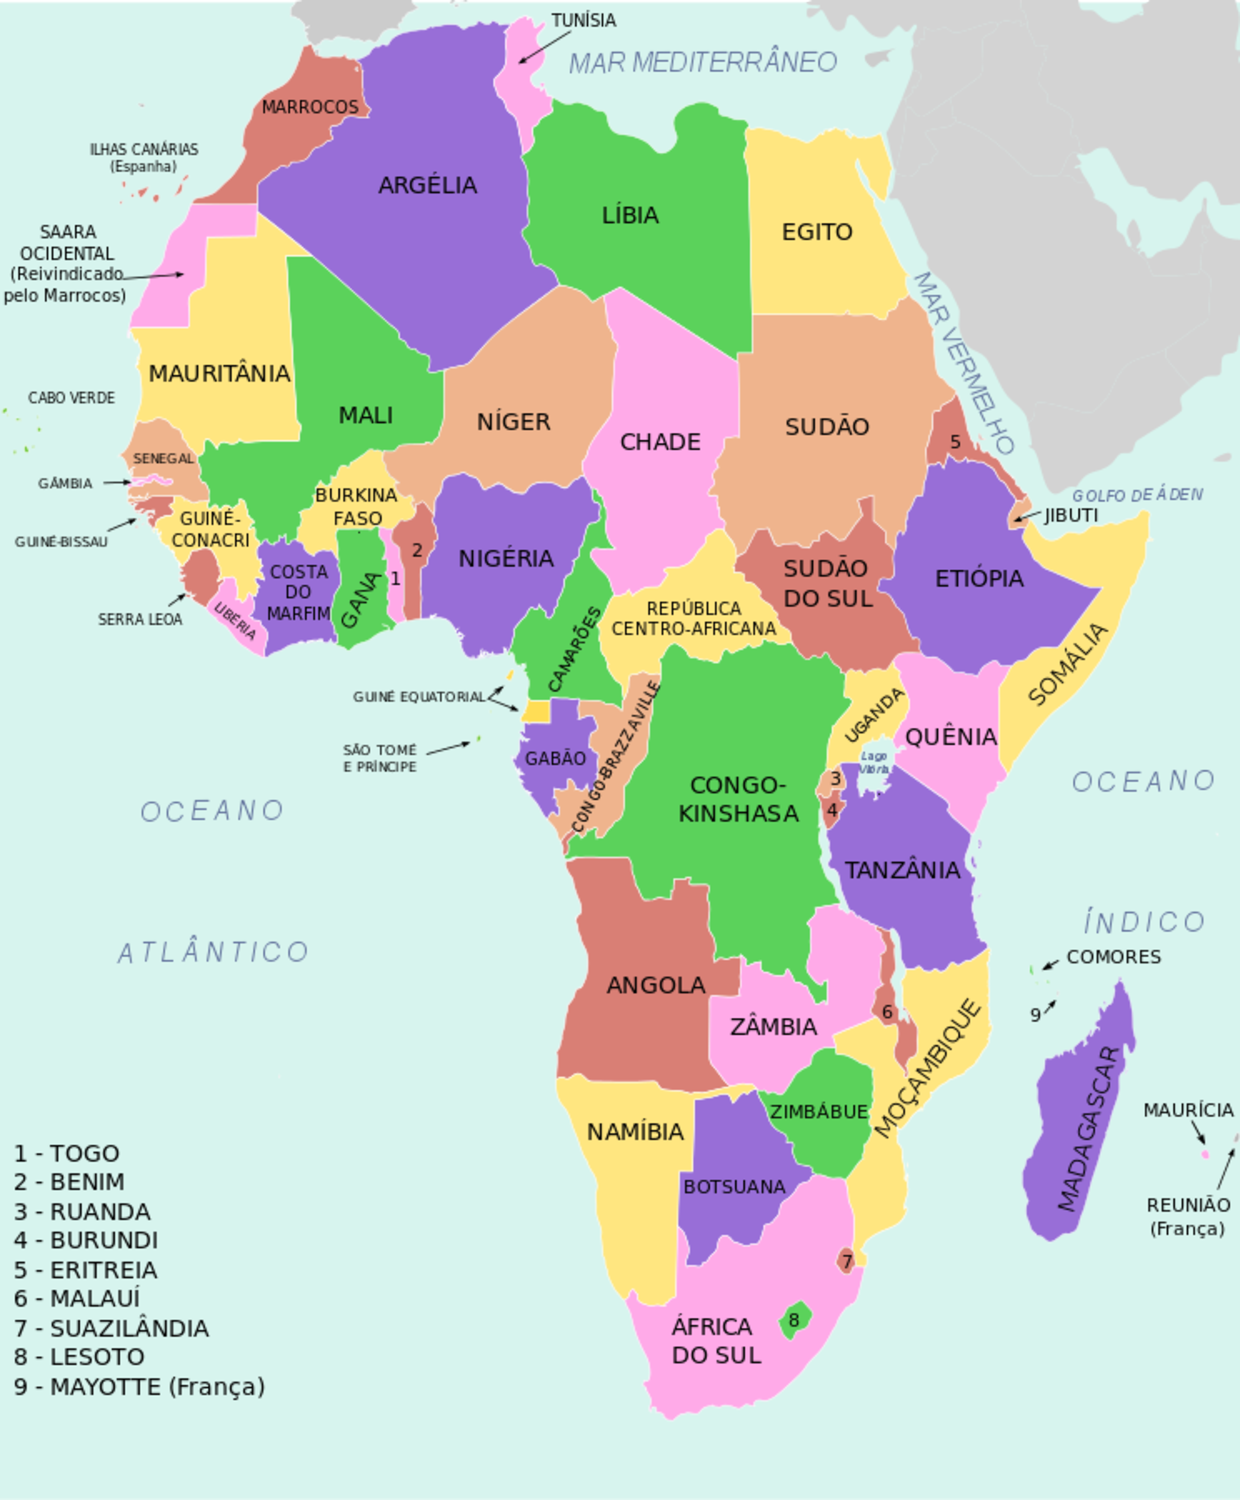
\includegraphics[width=0.55\linewidth]{../../inputs/images/africa_wikipedia.pdf}
  \end{figure}
\end{frame}

\begin{frame}
  \frametitle{África}
   \begin{itemize}
     \item Terceiro maior continente (extensão);
     \item Segundo maior em população, com 1,2 bilhões de habitantes (2015);
     \item 54 países (os mais pobres do mundo);
     \item Norte e Sul (África Subsariana - SSA) separados pelo deserto o Saara;
     \item Recente urbanização;
   \end{itemize}
\end{frame}

\begin{frame}
  \frametitle{Atividades de impactos na poluição do ar em cidades da SSA}
  \begin{itemize}
    \item População predominantemente rural, mas em transição;
    \item Excesso de vias não pavimentadas, mesmo nos centros das cidades;
    \item Alta taxa de crescimento populacional, sem a correspondente melhoria 
        na infraestrutura de serviços públicos;
    \item Emprego de queima de biomassa ou de lixo a céu aberto;
    \item Inexistência de sistemas de monitoramento de parâmetros ambientais, sistemáticos e em larga escala,
        realizados por agências de controle.
  \end{itemize}
\end{frame}

\begin{frame}
  \frametitle{}
  \begin{figure}[H]
    \centering
      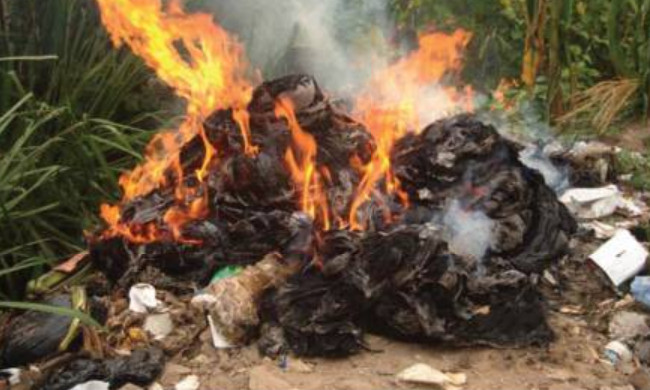
\includegraphics[width=0.5\linewidth]{../../inputs/images/zheng/arku3.jpeg}
      \caption{Queima de lixo a céu aberto em Nima. Por Raphael Arku 
             (reprodução autorizada pelo autor).\label{fig:nima_lixo}}
  \end{figure} 
\end{frame}

\begin{frame}
  \frametitle{Poluição do ar em cidades}
  Projeto Internacional: \\
  \textit{Poluição do Ar em Acra: Padrões temporais e espaciais e seus impactos sociais e econômicos.} \\ 
  coordenado pelo Prof. Dr. Majid Ezzati da \textit{Harvard School of Public Health}.
\end{frame}

\begin{frame}
  \frametitle{}
  \begin{figure}[H]
    \centering
    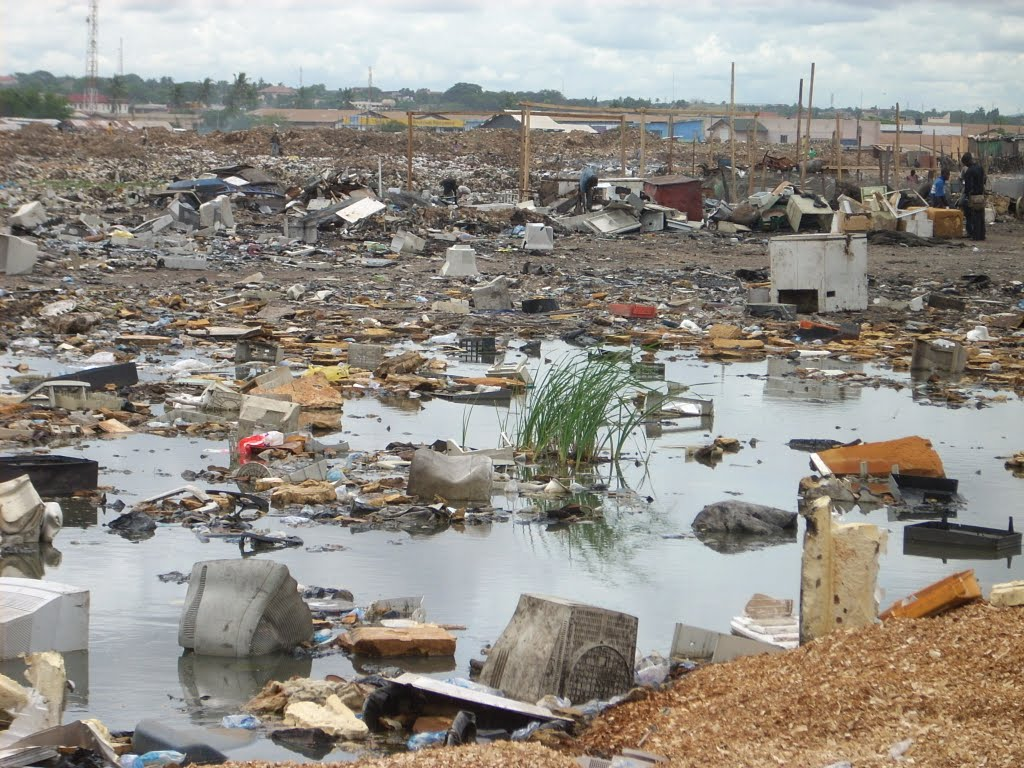
\includegraphics[width=0.5\textwidth]{../../inputs/images/ewaste_jack_caravano.jpg}
    \caption{Foto do depósito de lixo eletrônico (e-waste) situado no bairro 
             de Agbogbloshie em Acra. Fotografia de Jack Caravanos, 
             Professor da School of Public Health em Hunter College, CUNY
             Nova Iorque, Estado Unidos da América 
             (reprodução autorizada pelo autor). \label{fig:ewaste}}
  \end{figure}
\end{frame}

\begin{frame}
  \frametitle{}
  \begin{figure}[H]
    \centering
    \begin{subfigure}[b]{0.4\linewidth}
      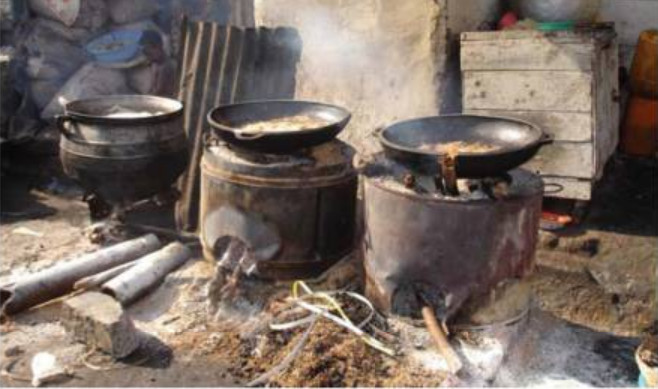
\includegraphics[width=\linewidth]{../../inputs/images/zheng/arku1.jpeg}
      \caption{Cozinha residencial em Nima adaptada para o uso de lenha.}
    \end{subfigure}%
    \hspace{0.5cm}
    \begin{subfigure}[b]{0.4\linewidth}
      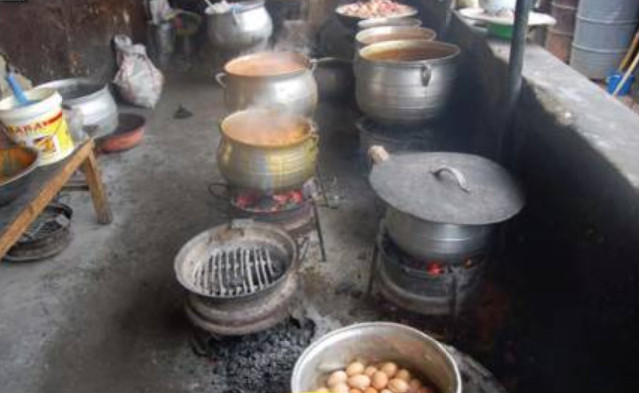
\includegraphics[width=\linewidth]{../../inputs/images/zheng/arku2.jpeg}
      \caption{Cozinha de comércio em Nima adaptada para o uso de carvão.}
    \end{subfigure}
    \caption{Fotos de cozinha residencial e comercial de Nima, por Raphael Arku 
             (reprodução autorizada pelo autor). \label{fig:nima}}
  \end{figure}
\end{frame}